\documentclass{article}
\usepackage[margin=1in]{geometry}
\usepackage[linesnumbered,ruled,vlined]{algorithm2e}
\usepackage{amsfonts}
\usepackage{amsmath}
\usepackage{amssymb}
\usepackage{amsthm}
\usepackage{enumitem}
\usepackage{fancyhdr}
\usepackage{hyperref}
\usepackage{minted}
\usepackage{multicol}
\usepackage{pdfpages}
\usepackage{standalone}
\usepackage[many]{tcolorbox}
\usepackage{tikz-cd}
\usepackage{transparent}
\usepackage{xcolor}
% \tcbuselibrary{minted}

\author{Nathan Solomon}

\newcommand{\fig}[1]{
    \begin{center}
        \includegraphics[width=\textwidth]{#1}
    \end{center}
}

% Math commands
\renewcommand{\d}{\mathrm{d}}
\DeclareMathOperator{\id}{id}
\DeclareMathOperator{\im}{im}
\DeclareMathOperator{\proj}{proj}
\DeclareMathOperator{\Span}{span}
\DeclareMathOperator{\Tr}{Tr}
\DeclareMathOperator{\tr}{tr}
\DeclareMathOperator{\ad}{ad}
\DeclareMathOperator{\ord}{ord}
%%%%%%%%%%%%%%% \DeclareMathOperator{\sgn}{sgn}
\DeclareMathOperator{\Aut}{Aut}
\DeclareMathOperator{\Inn}{Inn}
\DeclareMathOperator{\Out}{Out}
\DeclareMathOperator{\stab}{stab}

\newcommand{\N}{\ensuremath{\mathbb{N}}}
\newcommand{\Z}{\ensuremath{\mathbb{Z}}}
\newcommand{\Q}{\ensuremath{\mathbb{Q}}}
\newcommand{\R}{\ensuremath{\mathbb{R}}}
\newcommand{\C}{\ensuremath{\mathbb{C}}}
\renewcommand{\H}{\ensuremath{\mathbb{H}}}
\newcommand{\F}{\ensuremath{\mathbb{F}}}

\newcommand{\E}{\ensuremath{\mathbb{E}}}
\renewcommand{\P}{\ensuremath{\mathbb{P}}}

\newcommand{\es}{\ensuremath{\varnothing}}
\newcommand{\inv}{\ensuremath{^{-1}}}
\newcommand{\eps}{\ensuremath{\varepsilon}}
\newcommand{\del}{\ensuremath{\partial}}
\renewcommand{\a}{\ensuremath{\alpha}}

\newcommand{\abs}[1]{\ensuremath{\left\lvert #1 \right\rvert}}
\newcommand{\norm}[1]{\ensuremath{\left\lVert #1\right\rVert}}
\newcommand{\mean}[1]{\ensuremath{\left\langle #1 \right\rangle}}
\newcommand{\floor}[1]{\ensuremath{\left\lfloor #1 \right\rfloor}}
\newcommand{\ceil}[1]{\ensuremath{\left\lceil #1 \right\rceil}}
\newcommand{\bra}[1]{\ensuremath{\left\langle #1 \right\rvert}}
\newcommand{\ket}[1]{\ensuremath{\left\lvert #1 \right\rangle}}
\newcommand{\braket}[2]{\ensuremath{\left.\left\langle #1\right\vert #2 \right\rangle}}

\newcommand{\catname}[1]{{\normalfont\textbf{#1}}}

\newcommand{\up}{\ensuremath{\uparrow}}
\newcommand{\down}{\ensuremath{\downarrow}}

% Custom environments
\newtheorem{thm}{Theorem}[section]

\definecolor{probBackgroundColor}{RGB}{250,240,240}
\definecolor{probAccentColor}{RGB}{140,40,0}
\newenvironment{prob}{
    \stepcounter{thm}
    \begin{tcolorbox}[
        boxrule=1pt,
        sharp corners,
        colback=probBackgroundColor,
        colframe=probAccentColor,
        borderline west={4pt}{0pt}{probAccentColor},
        breakable
    ]
    \color{probAccentColor}\textbf{Problem \thethm.} \color{black}
} {
    \end{tcolorbox}
}

\definecolor{exampleBackgroundColor}{RGB}{212,232,246}
\newenvironment{example}{
    \stepcounter{thm}
    \begin{tcolorbox}[
      boxrule=1pt,
      sharp corners,
      colback=exampleBackgroundColor,
      breakable
    ]
    \textbf{Example \thethm.}
} {
    \end{tcolorbox}
}

\definecolor{propBackgroundColor}{RGB}{255,245,220}
\definecolor{propAccentColor}{RGB}{150,100,0}
\newenvironment{prop}{
    \stepcounter{thm}
    \begin{tcolorbox}[
        boxrule=1pt,
        sharp corners,
        colback=propBackgroundColor,
        colframe=propAccentColor,
        breakable
    ]
    \color{propAccentColor}\textbf{Proposition \thethm. }\color{black}
} {
    \end{tcolorbox}
}

\definecolor{thmBackgroundColor}{RGB}{235,225,245}
\definecolor{thmAccentColor}{RGB}{50,0,100}
\renewenvironment{thm}{
    \stepcounter{thm}
    \begin{tcolorbox}[
        boxrule=1pt,
        sharp corners,
        colback=thmBackgroundColor,
        colframe=thmAccentColor,
        breakable
    ]
    \color{thmAccentColor}\textbf{Theorem \thethm. }\color{black}
} {
    \end{tcolorbox}
}

\definecolor{corBackgroundColor}{RGB}{240,250,250}
\definecolor{corAccentColor}{RGB}{50,100,100}
\newenvironment{cor}{
    \stepcounter{thm}
    \begin{tcolorbox}[
        enhanced,
        boxrule=0pt,
        frame hidden,
        sharp corners,
        colback=corBackgroundColor,
        borderline west={4pt}{0pt}{corAccentColor},
        breakable
    ]
    \color{corAccentColor}\textbf{Corollary \thethm. }\color{black}
} {
    \end{tcolorbox}
}

\definecolor{lemBackgroundColor}{RGB}{255,245,235}
\definecolor{lemAccentColor}{RGB}{250,125,0}
\newenvironment{lem}{
    \stepcounter{thm}
    \begin{tcolorbox}[
        enhanced,
        boxrule=0pt,
        frame hidden,
        sharp corners,
        colback=lemBackgroundColor,
        borderline west={4pt}{0pt}{lemAccentColor},
        breakable
    ]
    \color{lemAccentColor}\textbf{Lemma \thethm. }\color{black}
} {
    \end{tcolorbox}
}

\definecolor{proofBackgroundColor}{RGB}{255,255,255}
\definecolor{proofAccentColor}{RGB}{80,80,80}
\renewenvironment{proof}{
    \begin{tcolorbox}[
        enhanced,
        boxrule=1pt,
        sharp corners,
        colback=proofBackgroundColor,
        colframe=proofAccentColor,
        borderline west={4pt}{0pt}{proofAccentColor},
        breakable
    ]
    \color{proofAccentColor}\emph{\textbf{Proof. }}\color{black}
} {
    \qed \end{tcolorbox}
}

\definecolor{noteBackgroundColor}{RGB}{240,250,240}
\definecolor{noteAccentColor}{RGB}{30,130,30}
\newenvironment{note}{
    \begin{tcolorbox}[
        enhanced,
        boxrule=0pt,
        frame hidden,
        sharp corners,
        colback=noteBackgroundColor,
        borderline west={4pt}{0pt}{noteAccentColor},
        breakable
    ]
    \color{noteAccentColor}\textbf{Note. }\color{black}
} {
    \end{tcolorbox}
}


\fancyhf{}
\setlength{\headheight}{24pt}

\date{\today}
\title{MATH 131B Homework \#4}

\begin{document}
\maketitle

\begin{prob}
    3.3.2
\end{prob}
Let $y_n = \lim_{x \rightarrow x_0, x \in E} f^{(n)}(x)$. For any $\varepsilon > 0$ and any $n \in \N$, there exists $\delta_n > 0$ such that $d(f^{(n)}(x), y_n) < \frac{\varepsilon}{4}$ whenever $d(x, x_0) < \delta_n$.
\par
Because the sequence of functions converges uniformly to $f$, there also exists $N \in \N$ such that $d(f(x), f^{(n)}(x)) < \frac{\varepsilon}{4}$ for any $n \geq N$ and any $x \in E$. By the triangle inequality, for this particular $N$,
\[ d(y_n, y_m) < d(y_n, f^{(n)}(x)) + d(f^{(n)}(x), f(x)) + d(f(x), f^{(m)}(x_0)) + d(f^{(m)}(x), y_m) < \varepsilon \]
whenever $d(x, x_0) < \min(\delta_n, \delta_m)$. That shows that $y_n$ is a Cauchy sequence, and since $Y$ is complete, that sequence converges to $y \in Y$.
\par
We want to show that $\lim_{x \rightarrow x_0, x \in E} f(x) = y$. This is fairly straighforward -- there exists $N \in \N$ such that $d(f(x), f^{(N)}(x)) < \frac{\varepsilon}{3}$ for any $x \in X$, $N$ can be further increased to ensure that $d(y_N, y) < \frac{\varepsilon}{3}$, and there exists $\delta_N > 0$ such that $d(f^{(N)}(x), y_N) < \frac{\varepsilon}{3}$ whenever $d(x, x_0) < \delta_N$. Then
\[ d(f(x), y) \leq d(f(x), f^{(N)}(x)) + d(f^{(N)}(x), y_N) + d(y_N, y) < \varepsilon, \]
meaning $f(x)$ converges to $y$. So in the equation we want to prove is true, both sides are equal to $y$.

\bigskip
\begin{prob}
    3.3.4
\end{prob}

\bigskip
\begin{prob}
    3.3.5
\end{prob}
Let $f^{(n)}: [0,1] \rightarrow [0,1]$ be the function which maps $x$ to $x^n$, and let $x^{(n)} = \sqrt[n]{\varepsilon} = \varepsilon^{1/n}$ for some $\varepsilon \in (0, 1)$.
\par
Then $f^{(n)}$ converges \textbf{pointwise} (but not uniformly) to $f$, where
\[ f(x) = \begin{cases}
    1 & x = 1 \\
    0 & x < 1,
\end{cases} \]
so $f(x^{(n)})=0$ for any $n \in \N$. However, $x^{(n)}$ converges to 1, and $f(1)=1\neq 0$.

\bigskip
\begin{prob}
    3.3.6
\end{prob}
Let $y_0$ be any point in $Y$. For each $n \in \N$, $f^{(n)}$ is bounded, meaning there exists $R_n \in \R$ such that $f^{(n)}(X) \subset B(y_0, R_n)$. Since the sequence of functions converges uniformly to $f$, for any $\varepsilon > 0$, there exists $N \in \N$ such that $d(f(x), f^{(n)}(x)) < \varepsilon$ whenever $n \geq N$ and $x \in X$. Therefore,
\[ d(f(x), y_0) \leq d(f(x), f^{(N)}(x)) + d(f^{(n)}(x), y_0) < \varepsilon + R_N, \]
so $f(X) \subset B(y_0, R_N + \varepsilon)$, meaning $f$ is bounded.

\bigskip
\begin{prob}
    3.5.1
\end{prob}
For each $i \in \left\{ 1, \dots, N \right\}$, define
\[ \norm{f^{(i)}}_\infty = \sup_{x \in X} \abs{f^{(i)}(x)} \]
Then for any $x \in X$,
\[ \left( \sum_{i=1}^N f^{(i)} \right) (x) = \sum_{i=1}^N \left( f^{(i)}(x) \right) \leq \sum_{i=1}^N \norm{f^{(i)}}_\infty, \]
which is the sum of finitely many real numbers, so the sum is bounded.
\par
If each $f^{(i)}$ is continuous at some $x_0 \in X$, then for any $\varepsilon > 0$, there exists $\delta_i > 0$ for every $i \in \left\{ 1, \dots, N \right\}$ such that
\[ d_X(f^{(i)}(x), f^{(i)}(x_0)) < \frac{\varepsilon}{N} \]
whenever $d(x, x_0) < \delta_i$. This implies
\[ d_X \left( \sum_{i=1}^N f^{(i)}(x), \sum_{i=1}^N f^{(i)}(x_0) \right) < \varepsilon, \]
so $\sum f^{(i)}$ is continuous at $x_0$. And of course, if each $f^{(i)}$ is continuous at every $x_0 \in X$, then so is $\sum f^{(i)}$.
\par
This proof would work just as easily if we had said ``uniformly continuous" instead of ``continuous". The only difference is that $\delta_i$ would need to ensure $d_X(f^{(i)}(x), f^{(i)}(x_0)) < \frac{\varepsilon}{N}$ for any $x, x_0 \in X$ which are distance less than $\delta_i$ apart, instead of for one specific $x_0 \in X$ and any $x$ withint a distance $\delta_i$ of $x_0$.

\bigskip
\begin{prob}
    3.5.2
\end{prob}

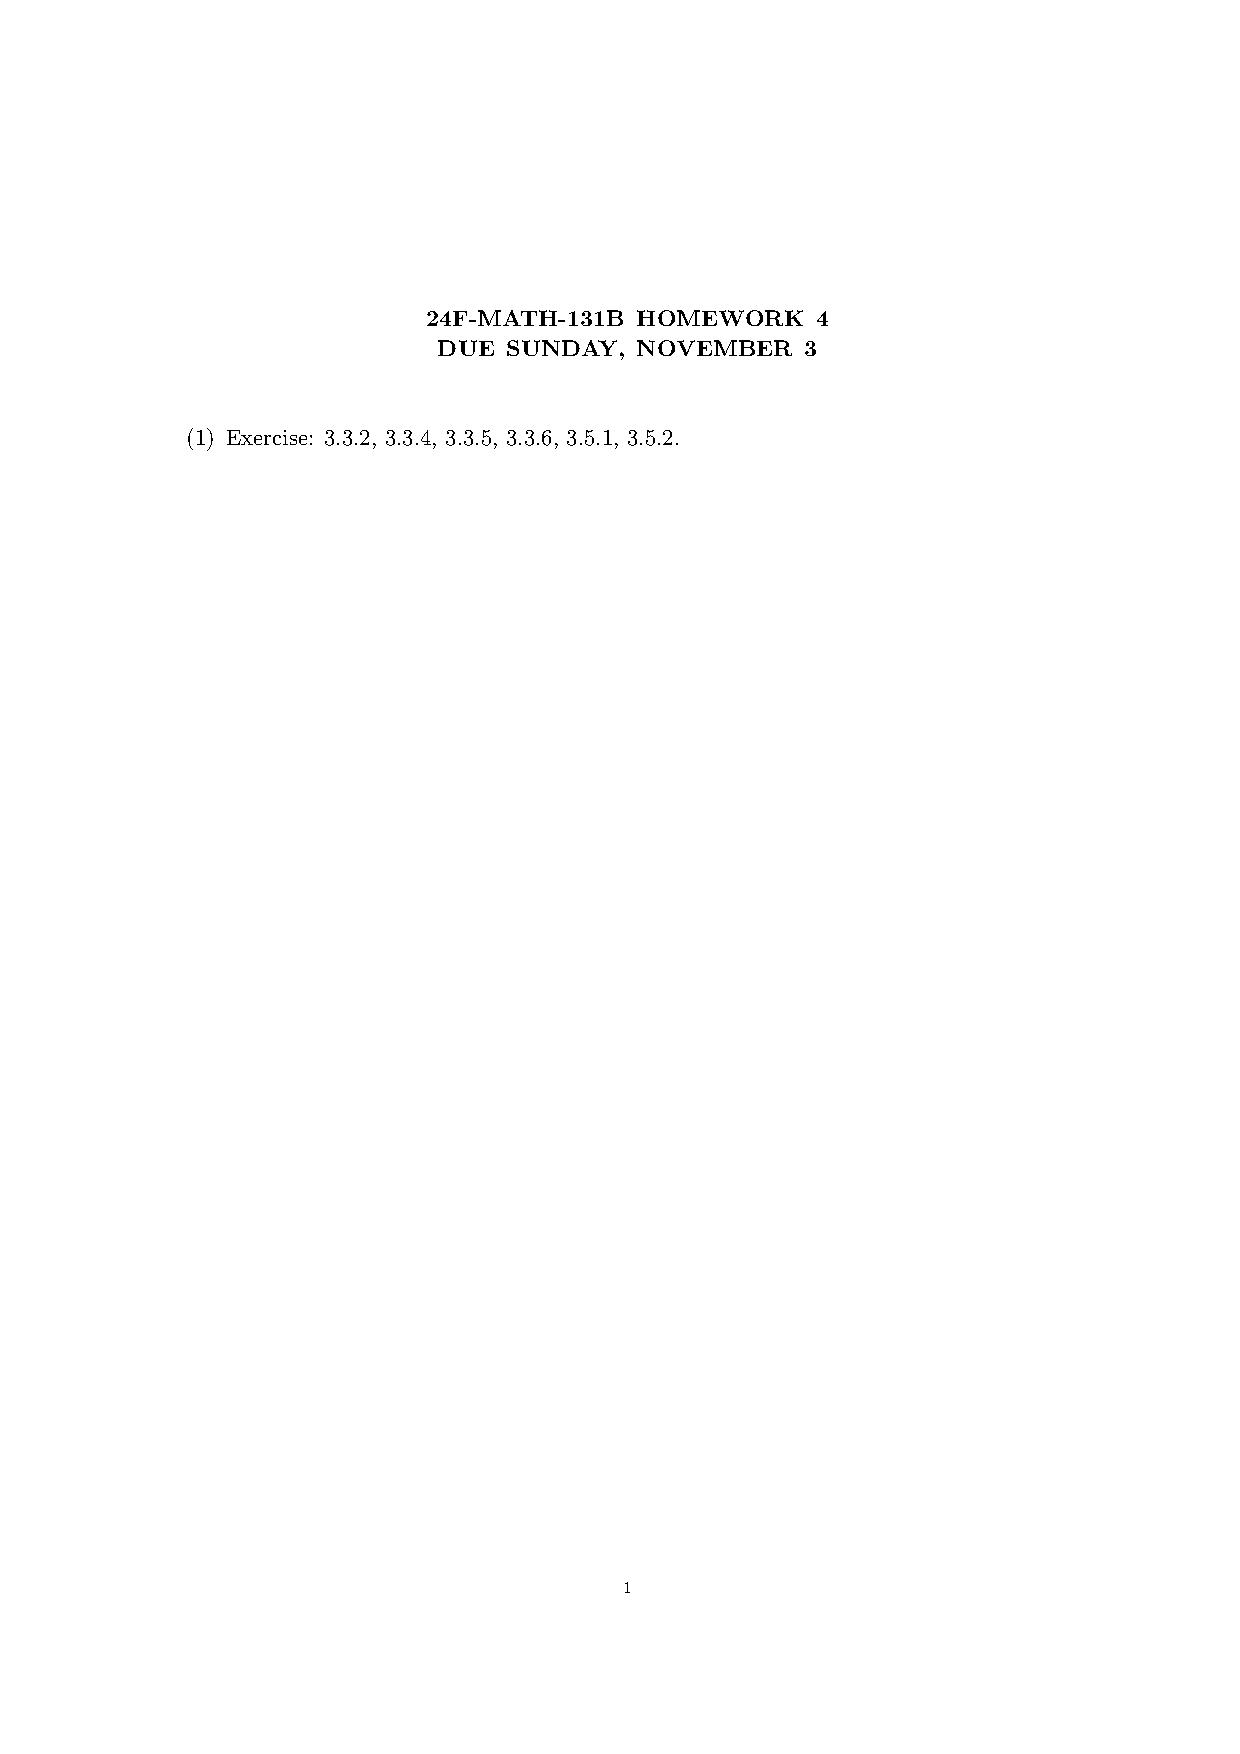
\includepdf[pages=-]{assignment.pdf}

\end{document}
